\chapter[Detection of copropagating beams for AWAKE]{Detection of copropagating beams for AWAKE}

AWAKE uses a copropagating electron and proton beam. The proton beam has a repetition rate of 10 Hz, while the proton beam from the SPS comes with time intervals in the order of the minute(s).

Outline of the problem:
CONS:
- two beams, sheilding each other
- not ideal proton beam, HF components

PROS:
- low repetition rate
- single pass device

\section[AWAKE instrumentation description]{AWAKE instrumentation description}

\subsection[Beamline and diagnostic]{Beamline and diagnostic}

Description of the SPS beamline, of the electron beamline and general other instrumentation installed (including the proton BPMs).

\subsection[Electron BPMs]{Electron BPMs}

The electron beam position monitoring system of the AWAKE facility was developed at TRIUMF\footnote{TRIUMF, Canada's Particle Accelerator Centre, Vancouver, BC, Canada, \url{https://www.triumf.ca/}}. It is composed by shorted stripline-type beam position monitor, and the readout electronics in charge of the signal processing.

\subsubsection{Beam position monitor}

Two types of beam position monitors are installed in the beamlines. In the electron beamline 40 mm aperture BPMs are used, while in the common beamline the 60 mm aperture model is used. The working principle is the same and they differ mostly on the mechanical dimensions. The coverage angle is 38 degrees, with a longitudinal lenght of 120 and 124 mm, respectively.

\subsubsection{Readout electronics}

GENERALITIES ON THE ELECTRONICS



\section[Signal generation]{Signal generation}

The signal is the convolution of the beam spectrum and the pickup response function (is it appropriate to speak of transfer function???). Some words on delta/sigma.

\subsection[Pickup response]{Pickup response}

Lobes and BPM details for shorted striplines

\subsection[Beam spectrum]{Beam spectrum}

In the AWAKE experiment a short electron bunch is propagating in close temporal and spacial proximity with a long proton bunch before entering the plasma cell. The beam parameters are reported in Tab.~\ref{beam_param_exp:tab}. Due to the different bunch length and charge, signals with different bandwidth and magnitude are expected from the two bunches. Figure~\ref{gauss_bunch} shows the time signals and the frequency spectrum of a 250 ps-sigma, 3e11 ppb proton bunch and a 1 ps-sigma, 600 pC electron bunch. From plot (b) it is trivial to see that around $\approx2$~GHz the power of the electron and proton bunch signal has equal strength. At lower frequencies the proton component dominates, while at higher frequencies the electron component has a higher power.

\begin{figure}[ht]
\centering
\subfigure[]
  {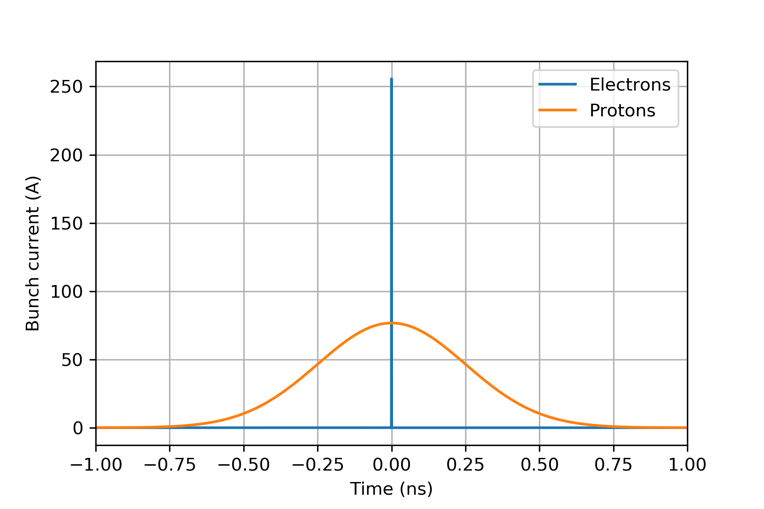
\includegraphics[width=6.5cm,height=5cm]{pictures/gauss_time}}
\hspace{3mm}
\subfigure[]
  {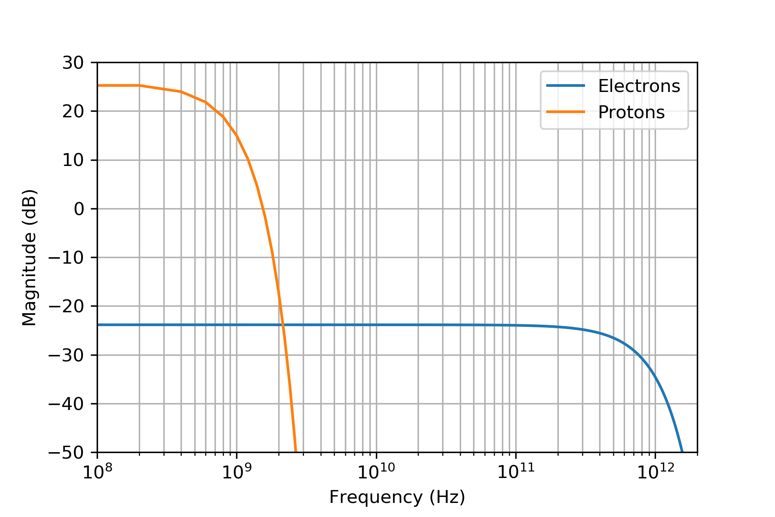
\includegraphics[width=6.5cm,height=5cm]{pictures/gauss_spectrum}}
\caption{The bunch in time (a) and frequency (b) with the paramters of the proton and electron bunch reported in Tab.~\ref{beam_param_exp:tab}.}
\label{gauss_bunch}
\end{figure}

Effect of a non-gaussian proton bunch. Extends more in spectrum.

It is reasonable to assume the electrons as gaussian (QUOTE)


\subsection[Two beam effect]{Two beam effect}

The spectrum is the sum of both, but different regions of the spectrum contain different level of information on the two beams.
